\documentclass{article}
\usepackage{ctable,microtype,amsmath,amssymb,graphicx,float}
\usepackage{siunitx}
\usepackage{xkeyval} 
\usepackage{cleveref}
\usepackage[utf8]{inputenc}
\usepackage[danish]{babel}
\usepackage{amsthm}
\setlength\parindent{0pt}
\setlength{\parskip}{1em}
\usepackage{fancyhdr}
\usepackage{dcolumn}
\usepackage[colorlinks,linkcolor=black,citecolor=blue,urlcolor=black]{hyperref}
\usepackage{setspace}
\usepackage[left=25mm, right=25mm, top=25mm, bottom=25mm]{geometry}
\usepackage{minted}
\usepackage{memhfixc}
\usepackage{subfiles}
\usepackage{csquotes}
\usepackage{xcolor}
\definecolor{LightGray}{gray}{0.9}
%\definecolor{DarkGray}{gray}{0.1}
%\pagecolor{DarkGray}
\usemintedstyle{borland}
%New colors defined below
\definecolor{codegreen}{rgb}{0,0.6,0}
\definecolor{codegray}{rgb}{0.5,0.5,0.5}
\definecolor{codepurple}{rgb}{0.58,0,0.82}
\definecolor{backcolour}{rgb}{0.95,0.95,0.92}
\title{Unit Tests}
\author{Simon Egeberg-201406253}
\usepackage[backend=biber,style=science,sorting=ynt,citestyle=science]{biblatex}
\addbibresource{references.bib}
\usepackage{graphicx}
\begin{document}
\maketitle
\begin{enumerate}
	\item Arrange
	\begin{itemize}
		\item Setup UUT og afhængigheder
	\end{itemize}
	\item Act
	\begin{itemize}
		\item Stimuler UUT (Dette er typisk selve testen)
	\end{itemize}
	\item Assert
	\begin{itemize}
		\item Check resultatet er som forventet
	\end{itemize}
\end{enumerate}
En unittest følger en meget bestemt setup. Ydermere er der nogle ting som skal stå klart før at en test kan få stemplet UNIT TEST.\

Lad og se på en konkret klasse, også se hvordan vi laver en unittest ud fra den.
\begin{listing}[H]
\begin{minted}[
frame=lines,tabsize=4,obeytabs,
framesep=2mm,
baselinestretch=1.2,
bgcolor=LightGray,
linenos
]{typescript}
class Subjects {
	private subjects: Subject[];
	constructor(private http: HttpClient) {
	}

	GetSubjects(): void {
		this.http.get(BASE_URL + '/api').subscribe(data => {
			this.subjects = data as Subject[];
		});
	}

	GetFirstSubject(): Subject {
		if(this.subjects) {
			return this.subjects[0];
		}
	}
}
\end{minted}
\caption{Angular klasse med http dependency}
\end{listing}

Startes der på at køre arrange act assert, så opstår der et problem. Sådan som det ser ud, så er \mintinline{typescript}|public subjects| nemlig tom. Så testes funktionen  \mintinline{typescript}|GetFirstSubject()| vil den aldrig retunere noget. 

En umiddelbar løsning på dette  ville være at give den et HttpClient modul som den vil have i constructoren, også kører funktionen GetSubjects(). Men dette skaber yderligere et problem. Der er ingen kontrol over hvad den funktion retunere. Derfor bliver vi en fake. (stub). 

I denne fake, som vi injector i constructoren kan der således laves en funktionen get som retunere et forudbestemt data array med Subjects. 

Nu har vi altså sat det hele op. Der er nemlig sørget for at subjects ikke er tom. Nu kan vi act og assert, og med ro i sindet være sikre på at det vi asserter mod, altid er det samme.

Dette er essencen af en unit test.


\begin{figure}[H]
	\centering
	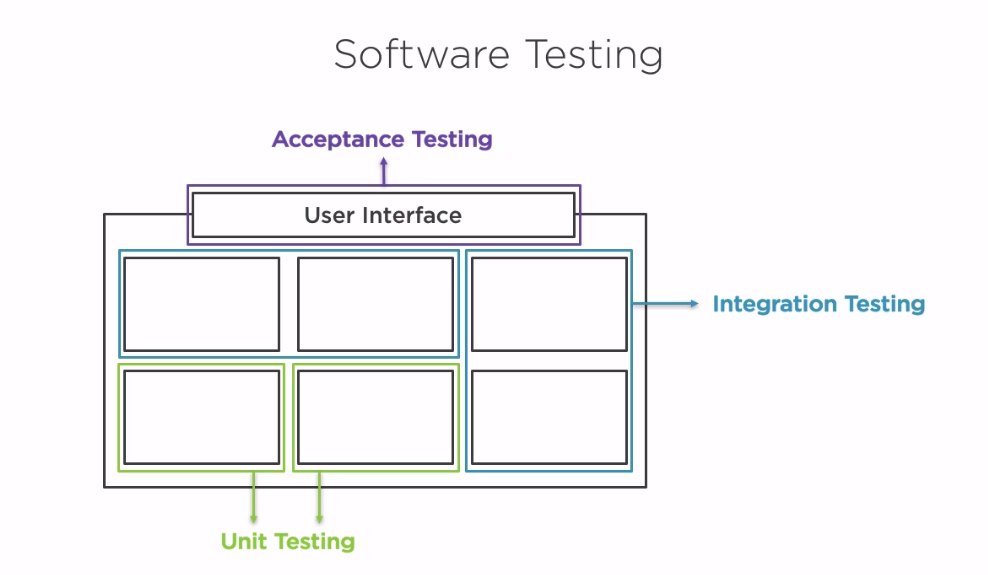
\includegraphics[width = \textwidth]{../softwaretesting.PNG}
\end{figure}
\end{document}